\section{Global Vector for Word Representation (GloVe)}
GloVe (Global Vector for Word Representation), bir kelime gömme yöntemidir.  Her bir kelime için vektörel temsiller oluşturur. Bu temsilleri oluştururken, kelimenin bağlamındaki ortaklıkları ve bağlamdaki sıklığını dikkate alır. Bu nedenle, kelimenin anlamını yakalamak için o kelimenin çevresindeki kelimelerin istatistiksel özelliklerini kullanır. Word2Vec'ten farklı olarak word2vec optimizasyon işlemini her seferinde yapar. Glove ise önce kaç defa geçtiğini hesaplar sonra optimizasyonu yapar yani her seferinde değil en sonda yapıyor.

\[J = \sum_{i,j=1}^{V} f(X_{ij}) \left( w_{i}^{T} \tilde{w_{j}} + b_{i} + \tilde{b_{j}} - \log X_{ij} \right)^2\]

\begin{itemize}
    \item $J$ = maliyet fonksiyonu.
    \item $V$ = kelime dağarcığının boyutu.
    \item $X_{ij}$ = kelime i ve j çiftinin birlikte geçme sayısı
    \item $w_{i}$ ve $w_{j}$ = kelime vektörleri
    \item $b_{i}$ ve $\tilde{b_{j}}$ = bias terimleri
    \item $f$ = ağırlık fonksiyonu
\end{itemize}

\begin{figure}[h]
    \centering
    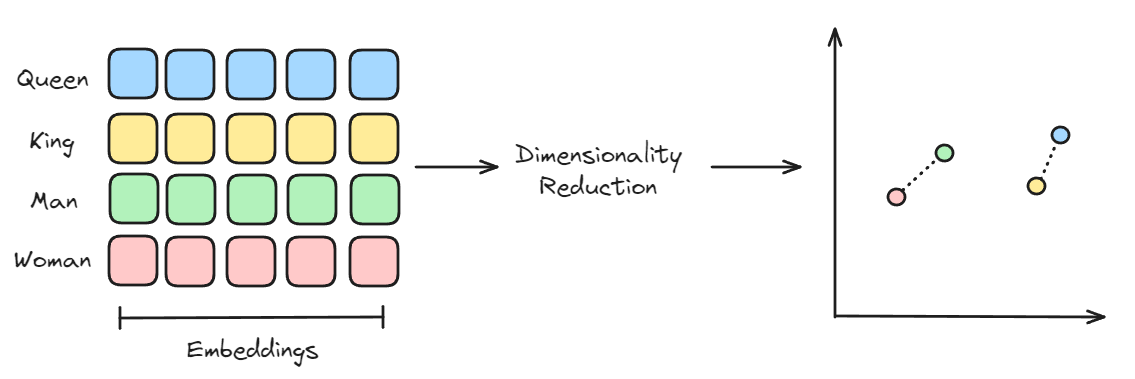
\includegraphics[width=1\textwidth]{images/glove.png}
    \caption{GloVe}
    \label{fig:enter-label}
\end{figure}

\newpage